Le modèle dont on s'est inspiré, présenté sur la figure~\ref{modele_original},
représente une vision du fonctionnement que pourrait avoir une conscience
artificielle. En se servant des travaux comme ceux de Freud et de Laborit, il permet de représenter la plupart des caractéristiques
d’une conscience humaine. 
\begin{figure}[H] 
\centering
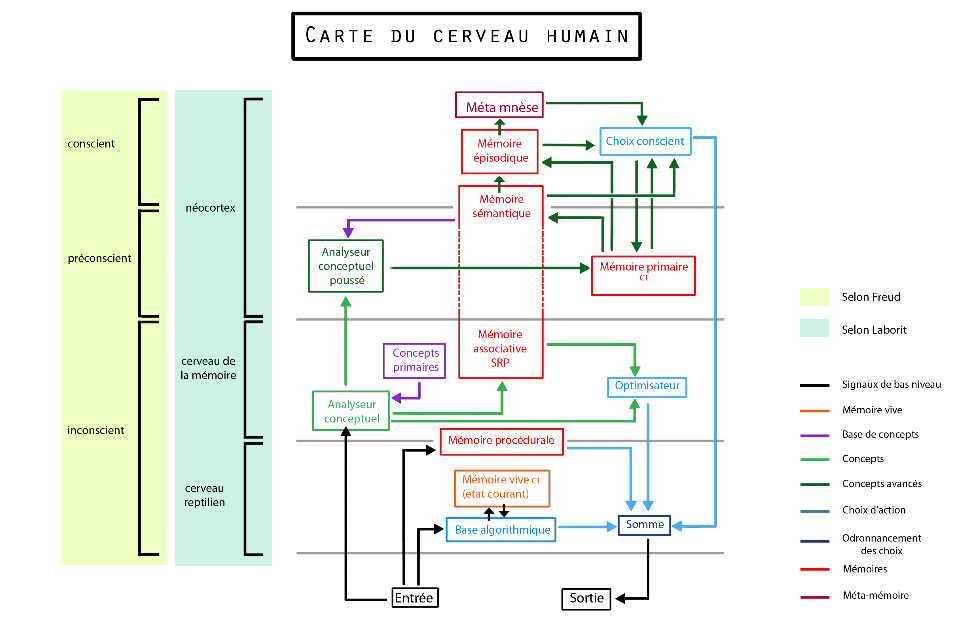
\includegraphics[width=\textwidth]{files/modele_original} 
\caption{Schéma du modèle de représentation de la conscience} 
\label{modele_original}
\end{figure}